\documentclass{templateNote}
\usepackage{tcolorbox}
\usepackage{pgfplots}
\usepackage{amsmath}
\usepackage{amssymb}
\usepackage{systeme}
\usepackage{empheq}
\usepackage{array}
\pgfplotsset{compat=1.18}

\begin{document}

\imagenlogo{img/LogoElNube.png}
\universidad{Universidad del Bío-Bío}
\titulo{Planos y Rectas} % Titulo
\asignatura{Algebra Lineal} % Asignatura
\autor{
    \indent
    Marcelo \textsc{Paz}
}   
\portada
\margenes % Crear márgenes


\section{Teoria}
\subsection{Ecuacion general del plano}
\indent
La ecuación general del plano es de la forma:
\begin{align*}
    Ax + By + Cz + D = 0
\end{align*}
Donde $A, B, C, D \in \mathbb{R}$.

\subsubsection{Importante}
Sean 2 planos cualquiera
\begin{align*}
    \pi_1: A_1x + B_1y + C_1z + D = 0 && \overrightarrow{n_1} = (A_1, B_1, C_1)\\
    \pi_2: A_2x + B_2y + C_2z + D = 0 && \overrightarrow{n_2} = (A_2, B_2, C_2)
\end{align*}
Son paralelos si:
\begin{align*}
    \overrightarrow{n_1} \parallel \overrightarrow{n_2} \iff \overrightarrow{n_1} = k\overrightarrow{n_2} \quad \text{, donde } k \in \mathbb{R}
\end{align*}
Son perpendiculares si:
\begin{align*}
    \overrightarrow{n_1} \perp \overrightarrow{n_2} \iff \overrightarrow{n_1} \cdot \overrightarrow{n_2} = 0
\end{align*}

Es \textbf{importante} aclarar que el producto cruz entre dos vectores, nos da como resultado un vector perpendicular a los vectores iniciales.
\begin{itemize}
    \item Si buscamos un plano perpendicular el vector resultante se toma como vector normal del plano.
    \item Si buscamos una recta perpendicular el vector resultante se toma como vector director de la recta.
\end{itemize}

\newpage
\subsubsection{Dado 3 puntos, encontrar la ecuacion general del plano}
\indent
Para encontrar la ecuación general del plano dados 3 puntos, se debe seguir los siguientes pasos:

Caso ejemplo:
\begin{align*}
    P_1 = (0, 0, 0) &&
    P_2 = (2, 0, 0) &&
    P_3 = (0, 2, 0)
\end{align*}
\begin{enumerate}
    \item Obtener 2 vectores del plano.
    \begin{align*}
        \overrightarrow{P_1P_2} = P_2 - P_1 = (2, 0, 0) &&
        \overrightarrow{P_1P_3} = P_3 - P_1 = (0, 2, 0)
    \end{align*}
    
    \item Calcular el producto cruz entre los 2 vectores, para determinar el (\textbf{vector normal}).
    \begin{align*}
        \overrightarrow{P_1P_2} \times \overrightarrow{P_1P_3} =  \begin{vmatrix} i & j & k \\ 2 & 0 & 0 \\ 0 & 2 & 0\end{vmatrix} = (0, 0, 4)  = \overrightarrow{n}&& \text{Vector normal}
    \end{align*}
    
    \item Usando el vector normal y uno de los puntos, se puede obtener la ecuación general del plano.
    \begin{align*}
        A(x-x_0) + B(y-y_0) + C(z-z_0) = 0 && \text{Ecuación general del plano} \\
    \end{align*}
    Donde $\overrightarrow{n} = (A, B, C)$ y $(x_0, y_0, z_0)$ es un punto cualquiera del plano.
    Remplazando:
    \begin{align*}
        0(x-0) + 0(y-0) + 4(z-0) = 0 && \text{Remplazamos los valores} \\
        \textrm{Asi,} \quad \pi: 4z = 0
    \end{align*}
\end{enumerate}

\begin{figure}[H]
    \centering
    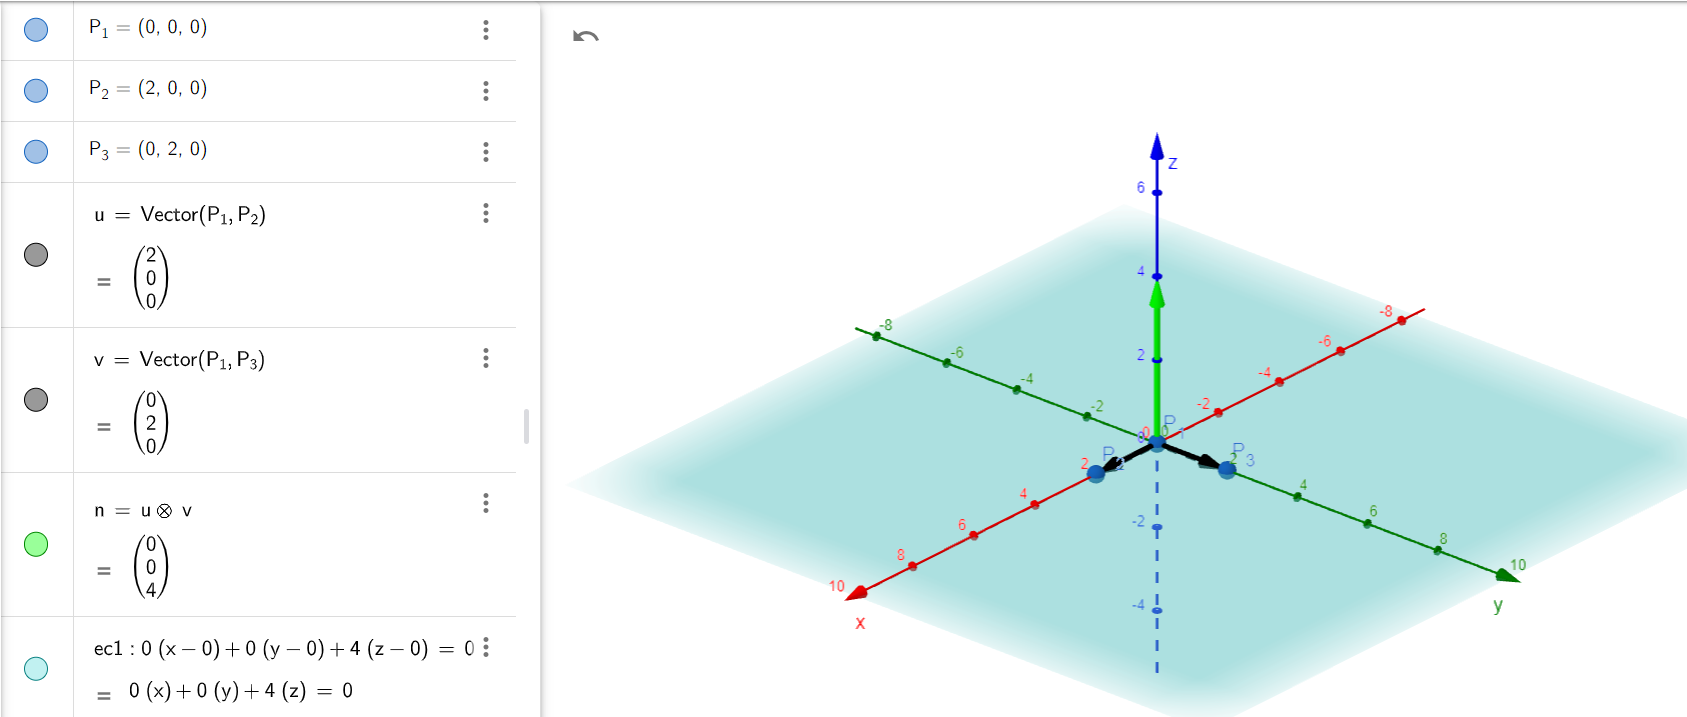
\includegraphics[width=\linewidth]{img/PlanoResultanteDado3Puntos.png}
    \caption{Plano Resultante dado 3 puntos}
\end{figure}
\newpage
\subsubsection{Dado un punto que pertenece al plano y dos planos ortogonales (perpendiculares), encontrar la ecuacion general del plano}
\indent
Para encontrar la ecuación general del plano dados un punto y dos planos ortogonales, se debe seguir los siguientes pasos:

Caso ejemplo:
\begin{align*}
    P_1 = (0, 0, 0) &&
    \pi_1: 2x + 2y + 2z + 2 = 0 &&
    \pi_2: x - y = 0
\end{align*}

\begin{enumerate}
    \item Obtener los vectores normales del plano 1 y 2.
    \begin{align*}
        \pi_1: 2x + 2y + 2z + 2 = 0 && \text{Ecuación general del plano} \\
        \overrightarrow{n} = (2, 2, 2) && \text{Vector normal}
    \end{align*}
    
    \begin{figure}[H]
        \begin{minipage}{0.5\textwidth}
          \centering
          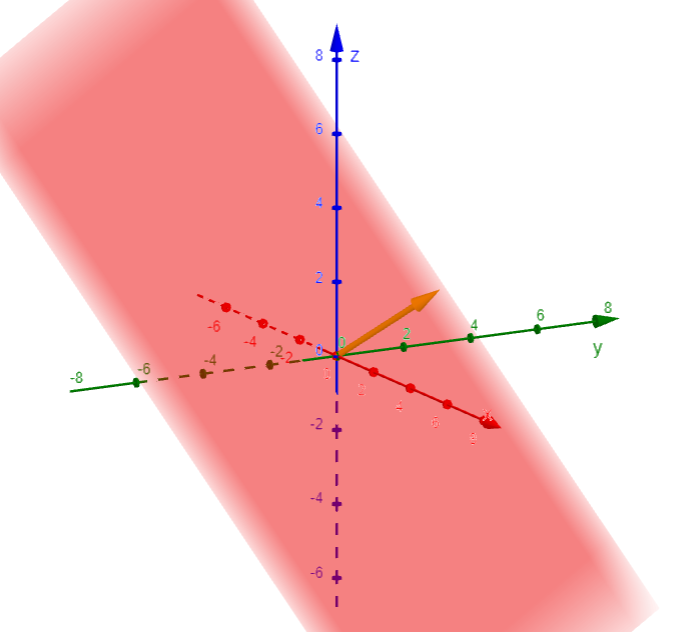
\includegraphics[width=0.9\linewidth]{img/Plano1.png}
          \caption{Plano 1}
        \end{minipage}
        \begin{minipage}{0.5\textwidth}
          \centering
          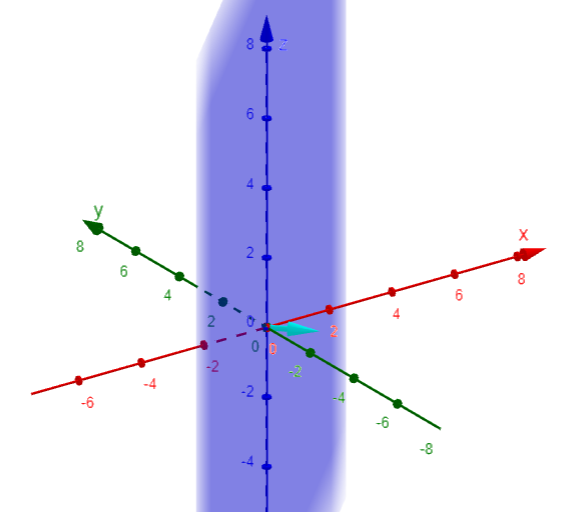
\includegraphics[width=0.9\linewidth]{img/Plano2.png}
          \caption{Plano 2}
        \end{minipage}
      \end{figure}

    \item Calcular el producto cruz entre los 2 vectores, para determinar el (\textbf{vector normal}).
    \begin{align*}
        \overrightarrow{n_1} \times \overrightarrow{n_2} =  \begin{vmatrix} i & j & k \\ 2 & 2 & 2 \\ 1 & -1 & 0\end{vmatrix} = (2, 2, -4)  = \overrightarrow{n}&& \text{Vector normal}
    \end{align*}

    \begin{figure}[H]
        \centering
        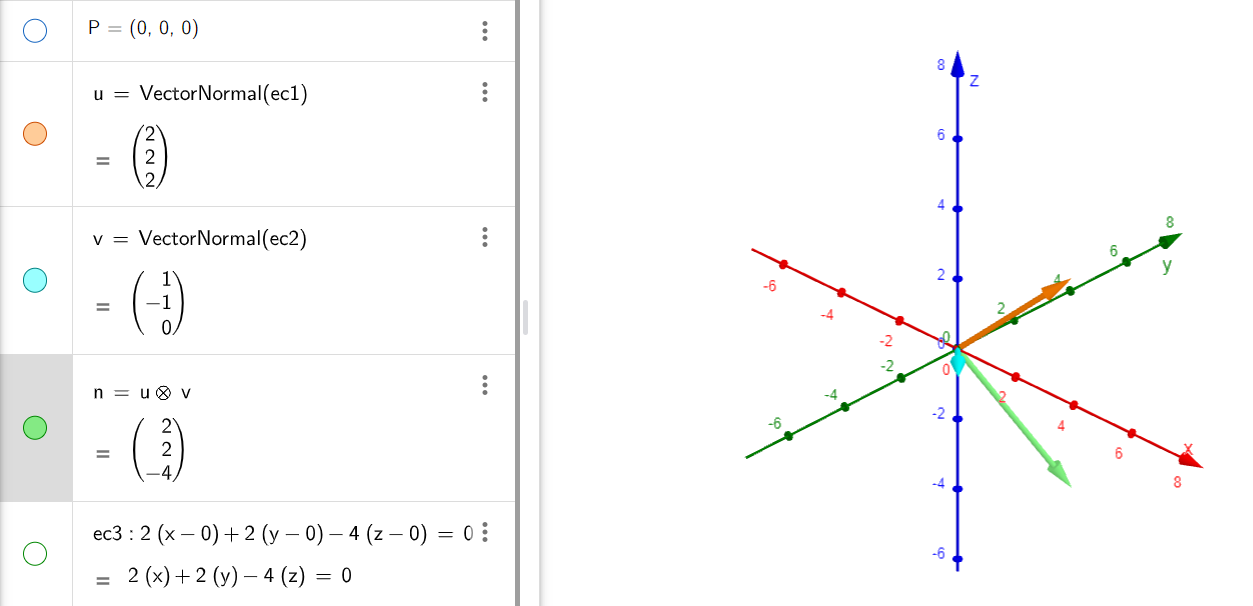
\includegraphics[width=0.8\linewidth]{img/ProductoVectorial.png}
        \caption{Producto cruz}
    \end{figure}
    \item Usando el vector normal y uno de los puntos, se puede obtener la ecuación general del plano.
    \begin{align*}
        2(x-0) + 2(y-0) + -4(z-0) = 0 && \text{Remplazamos los valores} \\
        \textrm{Asi,} \quad \pi: 2x + 2y - 4z = 0
    \end{align*}

    \begin{figure}[H]
        \centering
        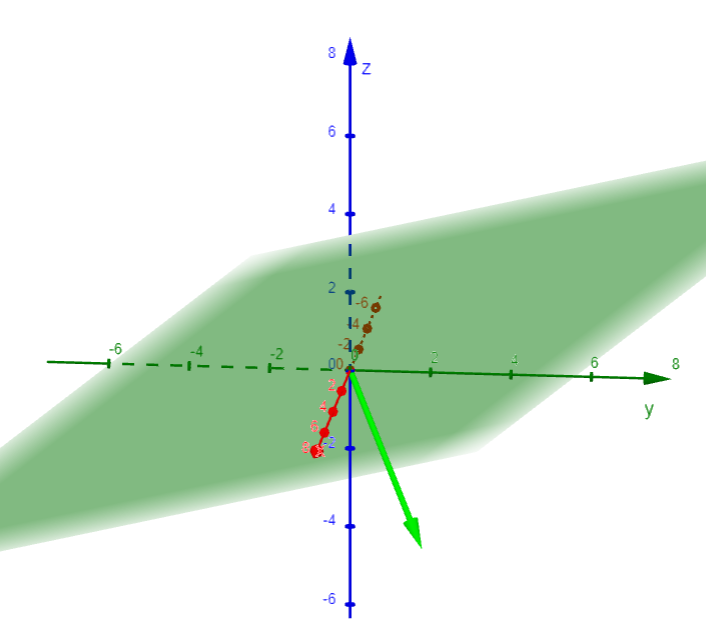
\includegraphics[width=0.8\linewidth]{img/PlanoResultante.png}
        \caption{Plano Resultante dado 1 punto y 2 planos ortogonales}
    \end{figure}

\end{enumerate}

\newpage
\section{Ecuacion de la recta}
\subsection{Ecuacion vectorial de la recta}
\indent
La ecuación vectorial de la recta es de la forma:
\begin{align*}
    \mathcal{L}(t) = \overrightarrow{P_1} + t\overrightarrow{v}
\end{align*}
Donde $\overrightarrow{P_1}$ es un punto cualquiera de la recta, $\overrightarrow{v}$ es el vector director de la recta y $t \in \mathbb{R}$.
*\textbf{Nota:} El vector normal es perpendicular, mientras que el vector director es paralelo.

\begin{figure}[H]
    \centering
    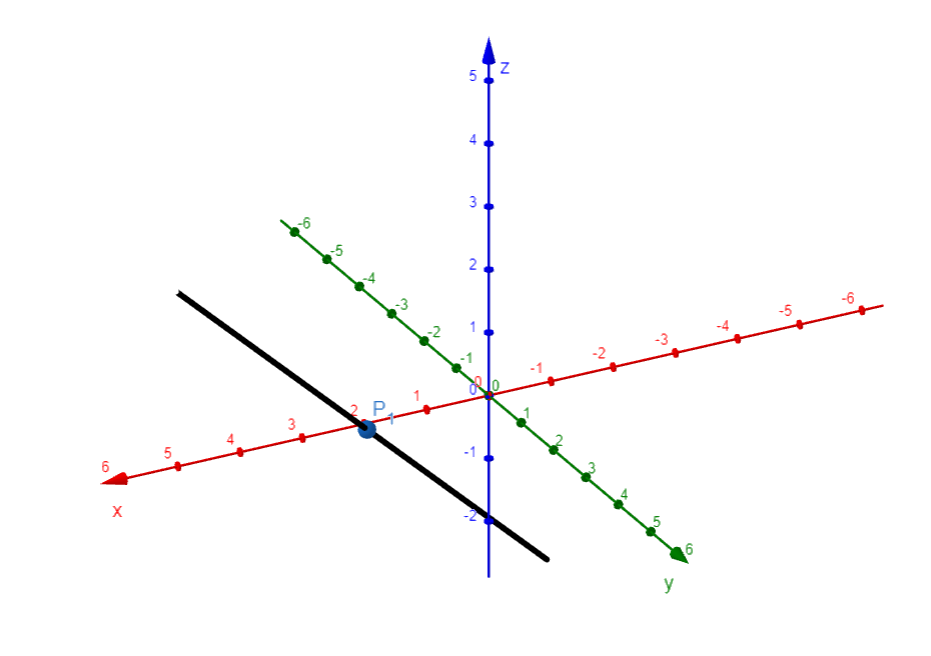
\includegraphics[width=0.6\linewidth]{img/Recta1.png}
    \caption{Recta vectorial}
\end{figure}

\subsection{Ecuacion parametrica de la recta}
\indent
La ecuación parametrica de la recta es de la forma:
\begin{align*}
    \mathcal{L}(t) = \begin{cases}
        x = x_0 + at \\
        y = y_0 + bt \\
        z = z_0 + ct
    \end{cases}
\end{align*}
Donde $P_1 = (x_0, y_0, z_0)$ es un punto cualquiera de la recta y $(a, b, c)$ es el vector director de la recta.

\subsection{Ecuacion simetrica de la recta}
\indent
La ecuación simetrica de la recta es de la forma:
\begin{align*}
    \mathcal{L} : \frac{x - x_0}{a} = \frac{y - y_0}{b} = \frac{z - z_0}{c}
\end{align*}
Donde $P_1 = (x_0, y_0, z_0)$ es un punto cualquiera de la recta y $(a, b, c)$ es el vector director de la recta, con $a \neq 0$, $b \neq 0$ y $c \neq 0$ 

\newpage
\subsection{Ecuacion de la recta dado la interseccion de dos planos}
\indent
Dado los planos:
\begin{align*}
    \pi_1: 2x + 5y + 4z + 15 = 0 && 
    \pi_2: -2x + 5y - 2z + 35 = 0
\end{align*}

\begin{enumerate}
    \item Determinamos los vectores normales de los planos.
    \begin{align*}
        \pi_1: 2x + 5y + 4z + 15 = 0 && \overrightarrow{n_1} = (2, 5, 4)\\
        \pi_2: -2x + 5y - 2z + 35 = 0 && \overrightarrow{n_2} = (-2, 5, -2)
    \end{align*}
    
    \item Determinamos el vector director de la recta, usando el producto cruz entre los vectores normales de los planos.
    \begin{align*}
        \overrightarrow{n_1} \times \overrightarrow{n_2} =  \begin{vmatrix} i & j & k \\ 2 & 5 & 4 \\ -2 & 5 & -2\end{vmatrix} = (-30,-4,20)  = \overrightarrow{v}&& \text{Vector director}
    \end{align*}
    
    \item Determinamos un punto de la recta, usando el sistema de ecuaciones de los planos.
    \begin{align*}
        \begin{cases}
            2x + 5y + 4z + 15 &= 0 \\
            -2x + 5y - 2z + 35 &= 0
        \end{cases} \tag*{\text{Sistema de ecuaciones}} \\
        \textrm{Podemos suponer que x,y,z = 0 :} \\
        \begin{cases}
            2x + 5y + 4(0) + 15 &= 0 \\
            -2x + 5y - 2(0) + 35 &= 0
        \end{cases} \tag*{\text{Remplazamos z = 0}} \\
        \begin{cases}
            2x + 5y + 15 &= 0 \\
            -2x + 5y + 35 &= 0
        \end{cases} \tag*{\text{Igualamos las ecuaciones}} \\
        2x + 5y + 15 &= -2x + 5y + 35 \tag*{\text{Restamos 5y}}\\
        4x &= 20 \tag*{\text{Dividimos por 4}}\\
        x &= 5 && \\
        \textrm{Remplazamos x = 5 en (1):} \\
        2(5) + 5y + 15 &= 0\\
        10 + 5y + 15 &= 0 \tag*{\text{Restamos 25}}\\
        5y &= -25 \tag*{text{Dividimos por 5}}\\
        y &= -5
    \end{align*}
    Asi obtenemos el punto $P_1 = (5, -5, 0)$

    \newpage
    \item Usando el punto y el vector director, podemos obtener la ecuación vectorial de la recta.
    \begin{align*}
        \mathcal{L}(t) &= \overrightarrow{P_1} + t\overrightarrow{v} \\
        \mathcal{L}(t) &= (5, -5, 0) + t(-30, -4, 20) \\
        \mathcal{L}(t) &= (5 - 30t, -5 - 4t, 20t)
    \end{align*}
\end{enumerate}

\begin{figure}[H]
    \centering
    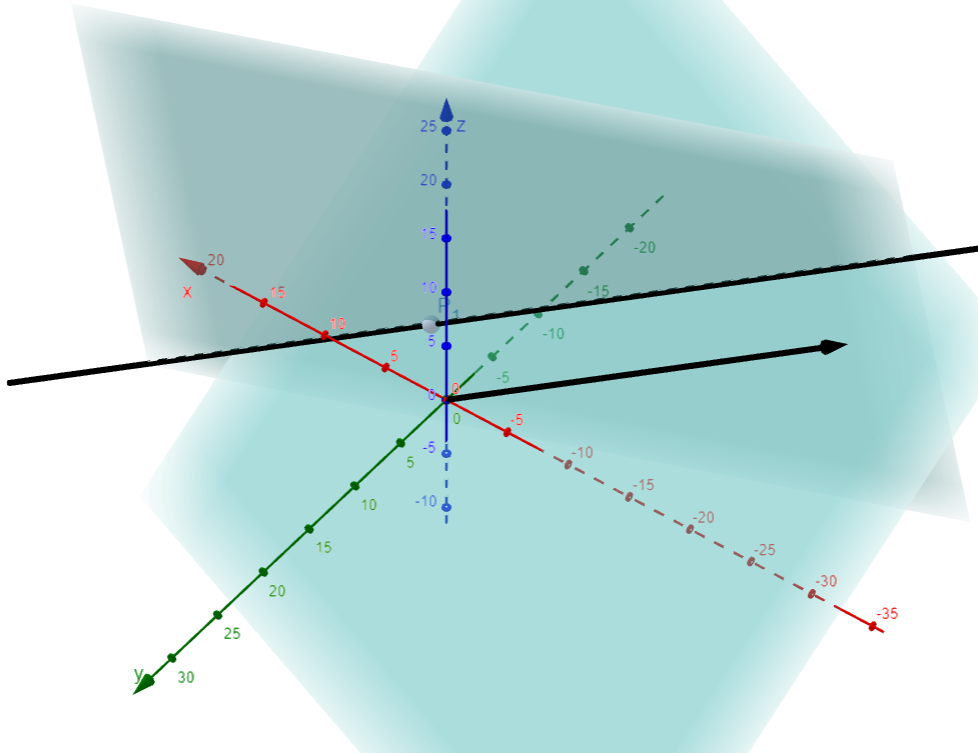
\includegraphics[width=0.6\linewidth]{img/RectaInterseccionP1.png}
    \caption{Recta dado la interseccion de dos planos perspectiva 1}
\end{figure}
\begin{figure}[H]
    \centering
    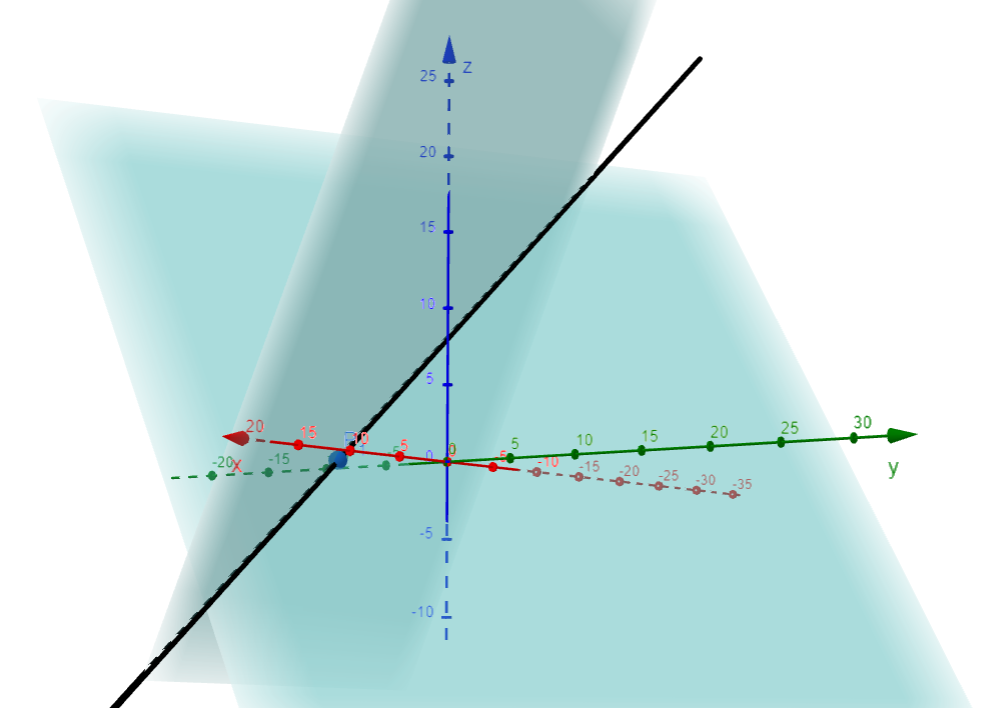
\includegraphics[width=0.6\linewidth]{img/RectaInterseccionP2.png}
    \caption{Recta dado la interseccion de dos planos perspectiva 2}
\end{figure}
\end{document}


